% LIP-PREPRINT-001
% Publication-ready LaTeX mirror of LIP_PREPRINT_001.md.
% Keep scientific claims and declarations synchronized with the canonical Markdown.
\documentclass[11pt]{article}

\usepackage[utf8]{inputenc}
\usepackage[T1]{fontenc}
\usepackage[a4paper,margin=22mm]{geometry}
\usepackage{amsmath,amssymb}
\usepackage{array,booktabs,tabularx}
\usepackage{caption}
\usepackage{enumitem}
\usepackage{xcolor}
\usepackage{microtype}
\usepackage{seqsplit}
\usepackage{tikz}
\usetikzlibrary{arrows.meta,positioning}
\usepackage{fancyhdr}
\usepackage{hyperref}
\usepackage{url}

\definecolor{lipnavy}{HTML}{16324F}
\definecolor{lipblue}{HTML}{2E6F9E}
\definecolor{lipteal}{HTML}{2A9D8F}
\definecolor{liporange}{HTML}{E68A2E}
\definecolor{lipred}{HTML}{C74440}
\definecolor{lipgray}{HTML}{6B7280}
\definecolor{lippale}{HTML}{EAF3F8}
\definecolor{lippaleorange}{HTML}{FFF0DF}

\hypersetup{
  colorlinks=true,
  linkcolor=lipnavy,
  citecolor=lipblue,
  urlcolor=lipblue,
  pdftitle={Receiver-Anchored Tests for Latent Communication},
  pdfauthor={Cristiano Silva},
  pdfsubject={LIP preprint: receiver-anchored evaluation of latent communication},
  pdfkeywords={latent communication, language-model agents, activation intervention, residual stream, causal evaluation}
}
\urlstyle{same}
\setlist[itemize]{leftmargin=1.5em,itemsep=0.25em,topsep=0.35em}
\setlist[enumerate]{leftmargin=1.7em,itemsep=0.25em,topsep=0.35em}
\setlength{\parindent}{0pt}
\setlength{\parskip}{0.55em}
\setlength{\tabcolsep}{5pt}
\renewcommand{\arraystretch}{1.13}
\emergencystretch=2em

\pagestyle{fancy}
\fancyhf{}
\fancyhead[L]{\small LIP - Latent Injection Protocol Preprint v0.1}
\fancyhead[R]{\small Cristiano Silva}
\fancyfoot[C]{\thepage}
\renewcommand{\headrulewidth}{0.3pt}

\newcommand{\yes}{\textbf{yes}}
\newcommand{\no}{no}

\title{\textbf{Receiver-Anchored Tests for Latent Communication}\\[0.35em]
\large Constant-Capacity Causal Localization and a Negative Cross-Model Result}
\author{Cristiano Silva\\
\normalsize Independent Researcher, Brazil\\
\small LIP --- Latent Injection Protocol}
\date{15 August 2026\\\small Version 0.1 --- Preprint}

\begin{document}

\maketitle

\begin{center}
\small
Correspondence: \href{mailto:ziwehdafe@gmail.com}{ziwehdafe@gmail.com}\\
DOI: \href{https://doi.org/10.5281/zenodo.21943476}{10.5281/zenodo.21943476}\\
Repository: \href{https://github.com/zigfreud/latent-llm-agent-communication}{github.com/zigfreud/latent-llm-agent-communication}\\
Manuscript CC BY 4.0 \(\cdot\) Code MIT
\end{center}

\begin{abstract}
Latent communication between language models is often evaluated as a single end-to-end problem: a sender state is mapped into a receiver, and downstream accuracy is treated as evidence for or against the whole idea. This conflates at least two questions. First, can the selected receiver-side carrier express task identity at all? Second, can a learned cross-model bridge reconstruct the task-specific receiver state well enough to affect generation? We formalize and apply a receiver-anchored evaluation protocol that separates these questions with receiver-native oracle replay, same-capacity identity shuffles, sealed task-level confirmation, and functional execution controls.

In a preregistered same-model study on 32 capability-screened MBPP tasks, a 24-position residual packet replayed through the first eight blocks of a pinned Llama-3-8B-Instruct receiver achieved 79/96 functional passes (82.29\%), while an equal-capacity same-stratum donor packet achieved 0/96. A constant-capacity \(2 \times 2 \times 2\) source factorial localized confirmed positive contributions to the terminal instruction core and function-name states (Holm-adjusted one-sided \(p = 0.0000699993\) for each); no positive boundary contribution was detected under the registered contrast.

We then tested a preregistered heterogeneous DeepSeek-Coder-1.3B-to-Llama-3-8B learned residual-packet bridge. All three primary replicas passed held-out retrieval and margin gates, and the receiver-native oracle anchor again succeeded (84/96 versus 0/96 shuffled). Nevertheless, learned matched and learned shuffled packets both achieved 1/288 functional passes, yielding a task-level identity effect of zero. The result is negative for this complete registered system. It shows that geometric separability on held-out development tasks was insufficient evidence of causal functional transport. The broader contribution is an auditable evaluation pattern for distinguishing carrier failure, bridge failure, and unsupported universality claims.
\end{abstract}

\noindent\textbf{Keywords:} latent communication; language-model agents; activation intervention; residual stream; cross-model alignment; causal evaluation; negative results; reproducible AI research

\section{Introduction}

Language-model agents normally communicate through text. Direct communication through activations, hidden states, or key-value caches could in principle avoid repeated decoding and preserve information that text serialization discards. The central technical challenge is not merely producing a continuous vector that resembles a target representation. It is demonstrating that task-specific information survives the complete sender-to-receiver path and changes downstream behavior for the intended reason.

An end-to-end failure is ambiguous. The source observation may omit the necessary information; the learned bridge may fail; the receiver-side insertion path may be incapable of expressing the task; or the functional evaluator may be insensitive or unsafe. Conversely, geometric success is also ambiguous. Low reconstruction error, high cosine similarity, or accurate task retrieval can coexist with negligible downstream causal effect.

This paper presents two registered studies from the LIP (Latent Injection Protocol) research program. Together they implement a receiver-anchored evaluation sequence:

\begin{enumerate}
  \item validate the receiver carrier with receiver-native matched and identity-shuffled packets;
  \item localize causally useful packet components while holding structural capacity constant;
  \item train and select cross-model bridges without consulting sealed confirmation tasks;
  \item compare learned matched packets with identity-shuffled, mean-scaffold, and norm-matched random controls under functional execution;
  \item make claims at the task level and stop when a preregistered gate fails.
\end{enumerate}

\begin{figure}[htbp]
\centering
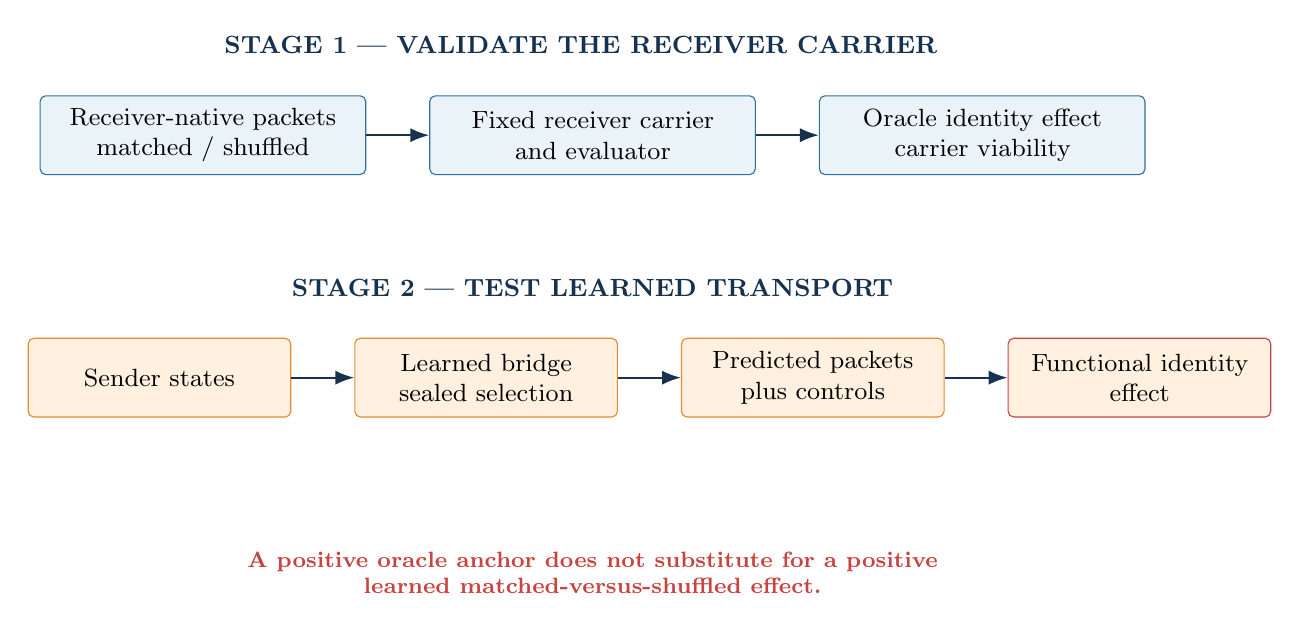
\begin{tikzpicture}[
  node distance=7mm and 8mm,
  box/.style={draw=lipblue,rounded corners=2pt,fill=lippale,align=center,minimum height=10mm,text width=39mm,font=\small},
  learned/.style={box,draw=liporange,fill=lippaleorange,text width=31mm},
  arr/.style={-{Latex[length=2.4mm]},thick,draw=lipnavy}
]
\node[font=\bfseries\small,text=lipnavy] (stageone) {STAGE 1 --- VALIDATE THE RECEIVER CARRIER};
\node[box,below=4mm of stageone,xshift=-48mm] (native) {Receiver-native packets\\matched / shuffled};
\node[box,right=of native] (carrier) {Fixed receiver carrier\\and evaluator};
\node[box,right=of carrier] (anchor) {Oracle identity effect\\carrier viability};
\draw[arr] (native) -- (carrier);
\draw[arr] (carrier) -- (anchor);

\node[font=\bfseries\small,text=lipnavy,below=12mm of carrier] (stagetwo) {STAGE 2 --- TEST LEARNED TRANSPORT};
\node[learned,below=4mm of stagetwo,xshift=-55mm] (sender) {Sender states};
\node[learned,right=of sender] (bridge) {Learned bridge\\sealed selection};
\node[learned,right=of bridge] (predicted) {Predicted packets\\plus controls};
\node[learned,right=of predicted,draw=lipred] (effect) {Functional identity\\effect};
\draw[arr] (sender) -- (bridge);
\draw[arr] (bridge) -- (predicted);
\draw[arr] (predicted) -- (effect);
\node[below=6mm of stagetwo,yshift=-24mm,text=lipred,font=\bfseries\footnotesize,align=center] {A positive oracle anchor does not substitute for a positive\\learned matched-versus-shuffled effect.};
\end{tikzpicture}
\caption{Receiver-anchored evaluation separates target-carrier viability from learned cross-model transport. All learned-side conditions reuse the validated carrier and functional evaluator.}
\label{fig:pipeline}
\end{figure}

The first study establishes that the selected receiver carrier can express task identity. A 24-position terminal packet copied from the receiver's own task-specific computation drives successful code generation, while an equally sized packet from another task does not. A source factorial further shows that the instruction core and function-name regions each contribute to the effect in an otherwise matched packet.

The second study asks whether a learned heterogeneous bridge can recreate that functionally useful state from a DeepSeek-Coder sender. Its development geometry is encouraging: three of three primary replicas pass joint, core, and name retrieval-margin gates. Its sealed functional result is not. Learned matched packets perform exactly like learned identity-shuffled packets at the task-clustered level.

The contribution is not the first proposal for latent communication. Earlier work communicates through activations, state trajectories, hidden states, and KV caches \cite{ramesh2025,tang2025,du2025,fu2025,wenzel2026,heo2026}. Our narrower contribution is a falsifiable evaluation pattern and a concrete result: a positive receiver-native oracle anchor can coexist with a zero learned identity effect, even after successful held-out geometric gates. This distinction matters when deciding whether a learned latent protocol has transported semantics or only organized representations.

\section{Related work and novelty boundary}

Ramesh and Li combine intermediate activations between language-model agents and report accuracy and efficiency gains \cite{ramesh2025}. State Delta Trajectory augments text communication with hidden-state changes \cite{tang2025}. Interlat communicates last hidden states and studies fully latent inter-agent exchange \cite{du2025}. Cache-to-Cache learns to project and fuse source and target KV caches \cite{fu2025}. Subsequent work has investigated sparse cross-architecture alignment and direct cache translation \cite{wenzel2026,heo2026}. A recent survey organizes this expanding area by representation, alignment, and receiver fusion \cite{liu2026}.

These systems differ in whether the sender and receiver share an architecture, whether text remains present, which internal object is transmitted, and how function is measured. The present paper does not claim priority over latent communication as a general idea, over activation injection, or over cross-model representation mapping. It instead focuses on three evaluation features used together:

\begin{itemize}
  \item a receiver-native oracle identity anchor before interpreting a learned bridge;
  \item matched-versus-shuffled interventions that preserve packet geometry and capacity;
  \item sealed, task-clustered functional confirmation that can invalidate a promising geometric development result.
\end{itemize}

The design is also related to causal abstraction and activation-intervention work \cite{geiger2021,zhang2023}. Those traditions emphasize that representational association and causal effect are different objects. LIP applies that distinction to a communication channel: the packet must not only be decodable or close to a teacher state; its task identity must alter receiver behavior relative to identity-destroying controls.

\section{Receiver-anchored evaluation}

\subsection{Two estimands, not one}

Let task \(i\) have a receiver-native task residual packet \(D_i\), an identity-shuffled donor packet \(D_{\pi(i)}\), a learned packet \(\widehat{D}_i\) predicted from the matching sender task, and a learned packet \(\widehat{D}_{\pi(i)}\) predicted from a same-stratum donor. Let \(Y(D)\) be a task-level functional outcome after receiver injection.

The receiver carrier effect is estimated by
\begin{equation}
\tau_{\mathrm{oracle}} = \operatorname{mean}_i\left[Y(D_i)-Y(D_{\pi(i)})\right].
\end{equation}

The learned identity effect is estimated by
\begin{equation}
\tau_{\mathrm{learned}} = \operatorname{mean}_i\left[Y(\widehat{D}_i)-Y(\widehat{D}_{\pi(i)})\right].
\end{equation}

A positive \(\tau_{\mathrm{oracle}}\) establishes that the selected receiver prompt, insertion path, packet geometry, and evaluation can express task identity on the tested population. It does not prove that a sender observation or learned bridge can reproduce the needed state. A positive learned effect requires the second contrast. If \(\tau_{\mathrm{oracle}}\) is positive and \(\tau_{\mathrm{learned}}\) is zero, the complete learned path failed despite a viable receiver carrier.

\subsection{Identity controls}

The principal negative control changes identity while preserving structure. Each shuffled packet comes from one other task in the same tokenizer-layout stratum. Donors are assigned by a derangement, so no task donates to itself. This control preserves packet shape, injected scalar count, insertion positions, insertion layers, and donor coherence.

The learned confirmation adds two controls. A mean scaffold contains only the training-set receiver mean. A random residual control samples an isotropic residual and rescales it to match the learned residual norm by layer. The four learned-side conditions therefore ask distinct questions:

\begin{itemize}
  \item learned matched versus learned shuffled: does the learned packet carry the correct task identity?
  \item learned matched versus mean scaffold: does the learned residual add function beyond the shared scaffold?
  \item learned matched versus norm-matched random: is success attributable to learned direction rather than residual magnitude alone?
\end{itemize}

\subsection{Functional and statistical units}

Generated Python is scored by task tests inside a hardened, network-isolated Linux namespace. Syntax-only scoring is explicitly ineligible for a semantic-transport claim. The task is the statistical unit. Multiple generation seeds and, where applicable, bridge replicas are averaged within task before contrasts. Bootstrap intervals resample tasks. One-sided sign-flip tests operate on paired task differences, and Holm correction controls each registered family \cite{holm1979}.

This prevents generation seeds, packet sites, or bridge replicas from being treated as independent task evidence. It also makes a zero identity effect interpretable: learned matched and shuffled conditions were compared on the same tasks under the same carrier and evaluator.

\section{Study A: constant-capacity causal localization}

\subsection{Research question}

The first study asks which components of a receiver-native terminal residual packet must preserve the target task's identity. It is an oracle replay study inside one pinned target model, not a learned inter-model bridge.

The population contains 32 MBPP test tasks \cite{austin2021}, selected before latent confirmation by a text-only capability screen. Sixteen tasks have two-token function names and sixteen have three-token names. The receiver is \texttt{NousResearch/Meta-Llama-3-8B-Instruct} at revision \texttt{53346005fb0ef11d3b6a83b12c895cca40156b6c}. Task states are captured from and replayed into the same receiver.

\subsection{Packet and factorial}

The packet spans 24 terminal prompt positions and the inputs to the first eight decoder blocks. Each packet is partitioned into:

\begin{itemize}
  \item \(C\), the terminal instruction core: 16 positions for two-token names or 15 for three-token names;
  \item \(N\), the required function-name states: two or three positions;
  \item \(B\), six fixed generation-boundary positions.
\end{itemize}

For each component, M denotes states matched to the target task and S denotes states from one same-stratum donor. The \(2 \times 2 \times 2\) conditions are MMM, SMM, MSM, MMS, SSM, SMS, MSS, and SSS. All contain exactly 24 populated positions. Two \(K=32\) replication controls plus neutral and text controls yield 12 conditions. With 32 tasks and three fresh generation seeds, confirmation contains 1,152 registered records.

The ordered gates first test full-\(K=32\) matched versus shuffled, then terminal-\(K=24\) MMM versus SSS. Only after both gates reject does a Holm family of seven component contrasts open. Three contribution contrasts replace one matched component in MMM. Four rescue contrasts return selected target components to an otherwise donor packet.

\subsection{Results}

Both ordered gates passed. Full-\(K=32\) matched replay achieved 85/96 functional passes (88.54\%) versus 0/96 shuffled. Terminal-\(K=24\) MMM achieved 79/96 (82.29\%) versus 0/96 SSS. The corresponding mean task-level effects were 0.885417 and 0.822917, each with one-sided Monte Carlo \(p = 0.0000099999\).

\begin{figure}[htbp]
\centering
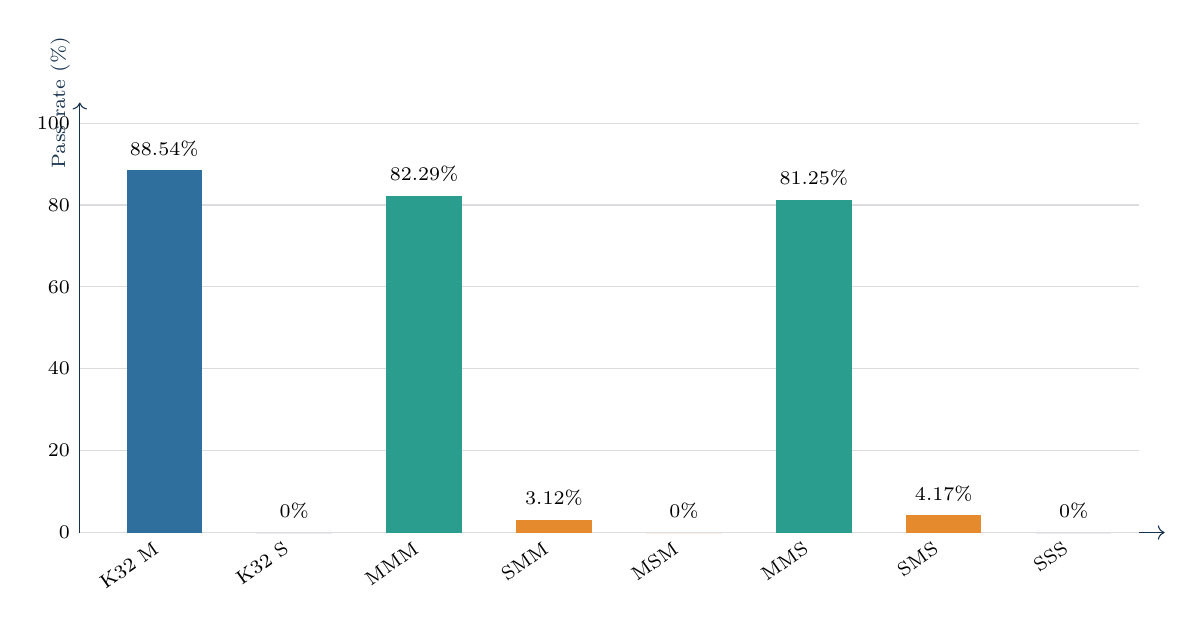
\begin{tikzpicture}[x=1.65cm,y=0.052cm,font=\scriptsize]
  \draw[->,lipnavy] (0,0) -- (8.35,0);
  \draw[->,lipnavy] (0,0) -- (0,105) node[above,rotate=90,anchor=south] {Pass rate (\%)};
  \foreach \y in {0,20,40,60,80,100} {
    \draw[lipgray!25] (0,\y) -- (8.15,\y);
    \node[left] at (0,\y) {\y};
  }
  \foreach \x/\lab/\v/\c in {0.65/{K32 M}/88.54/lipblue,1.65/{K32 S}/0/lipgray,2.65/{MMM}/82.29/lipteal,3.65/{SMM}/3.12/liporange,4.65/{MSM}/0/liporange,5.65/{MMS}/81.25/lipteal,6.65/{SMS}/4.17/liporange,7.65/{SSS}/0/lipgray} {
    \fill[\c] (\x-0.29,0) rectangle (\x+0.29,\v);
    \node[below,rotate=35,anchor=east] at (\x,-2) {\lab};
    \node[above] at (\x,\v+1) {\v\%};
  }
\end{tikzpicture}
\caption{Study A functional pass rates. M and S denote matched and same-stratum shuffled identity. The equal-capacity \(K=24\) factorial collapses when core or function-name identity is replaced, while the observed MMS rate remains near MMM.}
\label{fig:study-a}
\end{figure}

\begin{table}[htbp]
\centering
\caption{Study A functional pass rates.}
\label{tab:study-a-rates}
\small
\begin{tabularx}{\textwidth}{>{\raggedright\arraybackslash}X >{\raggedright\arraybackslash}X r r}
\toprule
Condition & Packet identity & Passes & Rate \\
\midrule
Neutral & no latent packet & 0/96 & 0.00\% \\
Task text & textual task prompt & 87/96 & 90.62\% \\
Full \(K=32\) matched & matched full packet & 85/96 & 88.54\% \\
Full \(K=32\) shuffled & donor full packet & 0/96 & 0.00\% \\
MMM & matched core, name, boundary & 79/96 & 82.29\% \\
SMM & donor core & 3/96 & 3.12\% \\
MSM & donor name & 0/96 & 0.00\% \\
MMS & donor boundary & 78/96 & 81.25\% \\
SMS & matched name only & 4/96 & 4.17\% \\
MSS / SSM / SSS & remaining donor controls & 0/288 & 0.00\% \\
\bottomrule
\end{tabularx}
\end{table}

The seven-test family confirmed two contributions:

\begin{table}[htbp]
\centering
\caption{Registered component contrasts in Study A.}
\label{tab:study-a-contrasts}
\scriptsize
\begin{tabularx}{\textwidth}{>{\raggedright\arraybackslash}X r c r l}
\toprule
Registered contrast & Mean diff. & 95\% task-bootstrap interval & Holm \(p\) & Result \\
\midrule
Core contribution: MMM -- SMM & 0.791667 & [0.645833, 0.916667] & 0.0000699993 & confirmed \\
Name contribution: MMM -- MSM & 0.822917 & [0.687500, 0.937500] & 0.0000699993 & confirmed \\
Boundary contribution: MMM -- MMS & 0.010417 & [0.000000, 0.031250] & 1.0 & not confirmed \\
Core-only rescue: MSS -- SSS & 0.000000 & [0.000000, 0.000000] & 1.0 & not confirmed \\
Name-only rescue: SMS -- SSS & 0.041667 & [0.000000, 0.114583] & 1.0 & not confirmed \\
Boundary-only rescue: SSM -- SSS & 0.000000 & [0.000000, 0.000000] & 1.0 & not confirmed \\
Name-plus-boundary rescue: SMM -- SSS & 0.031250 & [0.000000, 0.093750] & 1.0 & not confirmed \\
\bottomrule
\end{tabularx}
\end{table}

The factorial surface is conjunctive. Replacing only function-name identity reduced observed success from 82.29\% to 0\%; replacing only core identity reduced it to 3.12\%. Neither component alone rescued an otherwise donor packet. Replacing only boundary identity left 78/96 passes, one below MMM. Because equivalence and non-inferiority were not preregistered, this near-equality does not establish universal boundary irrelevance. It establishes only that the registered positive boundary-contribution contrast did not reject.

Descriptive geometry agrees with the intervention after the packet is decomposed. Common function-name positions had a mean task-signal fraction of 0.7050, compared with 0.5875 for common core positions and 0.0297 for boundary positions. Mean residual norms were comparable (2.3281, 2.2025, and 1.9974, respectively), illustrating why magnitude is not a task-information score.

\section{Study B: learned heterogeneous transport}

\subsection{Sender, receiver, and packet bridge}

The second study fixes a heterogeneous path from \texttt{deepseek-ai/deepseek-coder-1.3b-base} at revision \texttt{e5babb80b8539a4e85dd2418c0ee611522276987} to the same pinned Llama-3-8B-Instruct receiver \cite{grattafiori2024,guo2024}. The sender observation has shape 24 layers \(\times\) 32 terminal positions \(\times\) 2048 features. Each sender state is projected to width 512, normalized, augmented with learned layer and position embeddings, and flattened into 768 source-memory sites.

Thirty-two learned protocol queries pass through two pre-normalized Transformer decoder blocks with eight-head cross-attention to produce a fixed \(32 \times 512\) LIP code. The receiver decoder forms \(8 \times 24\) receiver-site queries, cross-attends them to that code in two further blocks, and projects each decoded site to a normalized residual of width 4096. At inference, training-only site scales and the mean scaffold reconstruct the absolute packet as \(\widehat H = \mu_{\mathrm{train}} + \sigma \odot \widehat{\widetilde\Delta}\) before injection into the residual inputs of receiver blocks 0 through 7.

\begin{figure}[htbp]
\centering
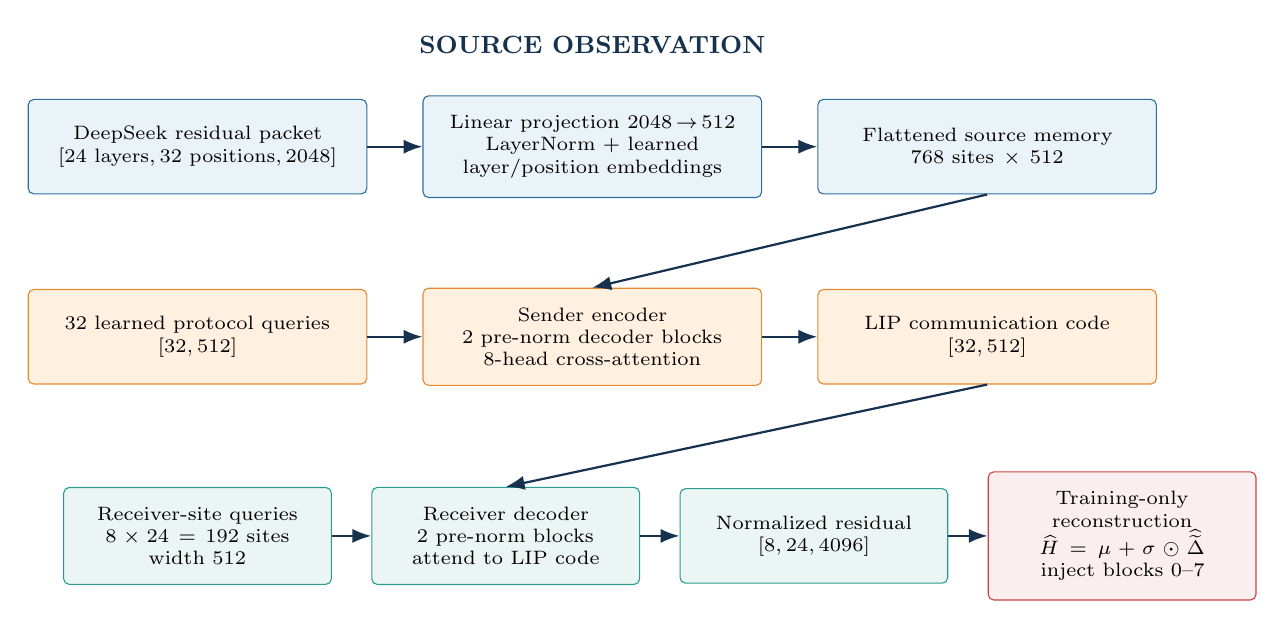
\begin{tikzpicture}[
  node distance=7mm and 7mm,
  base/.style={rounded corners=2pt,align=center,minimum height=12mm,inner sep=2.5mm,font=\scriptsize},
  source/.style={base,draw=lipblue,fill=lippale,text width=38mm},
  bridge/.style={base,draw=liporange,fill=lippaleorange,text width=38mm},
  receiver/.style={base,draw=lipteal,fill=lipteal!10,text width=29mm},
  output/.style={receiver,draw=lipred,fill=lipred!9},
  arr/.style={-{Latex[length=2.4mm]},thick,draw=lipnavy}
]
\node[source] (source) {DeepSeek residual packet\\\([24\ \text{layers},32\ \text{positions},2048]\)};
\node[source,right=of source] (projection) {Linear projection \(2048\!\to\!512\)\\LayerNorm + learned layer/position embeddings};
\node[source,right=of projection] (memory) {Flattened source memory\\\(768\ \text{sites}\times512\)};
\node[font=\bfseries\small,text=lipnavy,above=4mm of projection] {SOURCE OBSERVATION};
\draw[arr] (source) -- (projection);
\draw[arr] (projection) -- (memory);

\node[bridge,below=12mm of source] (queries) {32 learned protocol queries\\\([32,512]\)};
\node[bridge,right=of queries] (encoder) {Sender encoder\\2 pre-norm decoder blocks\\8-head cross-attention};
\node[bridge,right=of encoder] (code) {LIP communication code\\\([32,512]\)};
\draw[arr] (queries) -- (encoder);
\draw[arr] (memory.south) -- (encoder.north);
\draw[arr] (encoder) -- (code);

\node[receiver,below=13mm of queries] (receiverqueries) {Receiver-site queries\\\(8\times24=192\) sites\\width 512};
\node[receiver,right=5mm of receiverqueries] (decoder) {Receiver decoder\\2 pre-norm blocks\\attend to LIP code};
\node[receiver,right=5mm of decoder] (residual) {Normalized residual\\\([8,24,4096]\)};
\node[output,right=5mm of residual] (reconstruct) {Training-only reconstruction\\\(\widehat H=\mu+\sigma\odot\widehat{\widetilde\Delta}\)\\inject blocks 0--7};
\draw[arr] (receiverqueries) -- (decoder);
\draw[arr] (code.south) -- (decoder.north);
\draw[arr] (decoder) -- (residual);
\draw[arr] (residual) -- (reconstruct);
\end{tikzpicture}
\caption{Architecture of the registered query-conditioned nonlinear bridge used in Study B. The diagram describes the tested system and its training-only scaffold reconstruction; it does not imply successful functional semantic transport.}
\label{fig:bridge-architecture}
\end{figure}

All splits are by task: 256 MBPP train tasks, 32 development-selection tasks, 32 disjoint development-gate tasks, and 32 sealed confirmation tasks. The confirmation cohort is balanced across the same two function-name strata and is disjoint from the preceding oracle-confirmation cohort and all bridge train/development tasks.

Three systems are trained with three registered seeds: a component-contrastive nonlinear bridge, the same nonlinear bridge with centered regression only, and a structured linear regression baseline. Checkpoint selection consults development-selection only. The selected checkpoint is opened once on development-gate. A primary replica passes only if joint, core, and name task-retrieval margins are positive under one Holm family. Confirmation opens only if at least two of three primary replicas pass.

All three component-contrastive replicas passed this gate. All three structured-linear replicas also passed; centered regression passed zero of three. The registered primary aggregate rule therefore opened confirmation. This is an important intermediate observation, but it is not a functional result.

\subsection{Sealed functional confirmation}

Confirmation contains 1,344 complete cells. Neutral, text-only, oracle-matched, oracle-shuffled, and mean-scaffold conditions each contain 96 generations. Learned matched, learned shuffled, and norm-matched random conditions each contain 288 generations because they cross 32 tasks, three bridge replicas, and three generation seeds.

The receiver-native oracle anchor passed again: oracle matched achieved 84/96 (87.50\%), while oracle shuffled achieved 0/96. The carrier, receiver prompt, and task evaluator can therefore express the required identity on this cohort.

The learned bridge failed its primary functional family. Learned matched and learned shuffled each achieved 1/288 (0.3472\%). After averaging replicas and generation seeds within task, their mean paired difference was exactly zero, their interval was [0, 0], and the one-sided \(p\)-value was 1.0.

\begin{figure}[htbp]
\centering
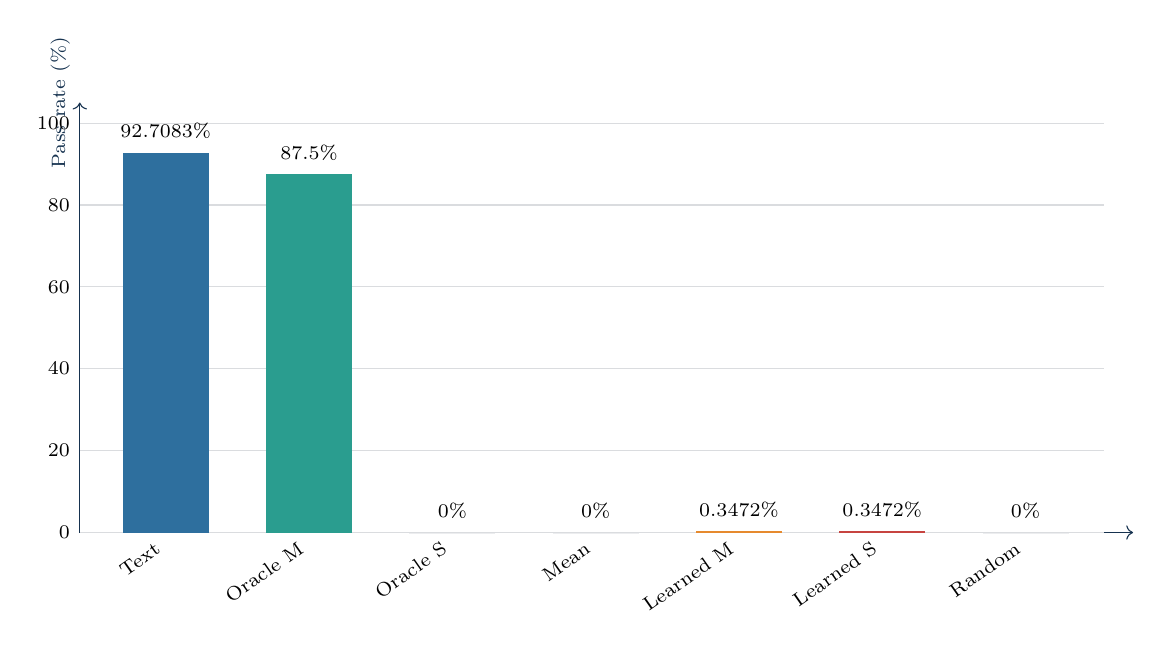
\begin{tikzpicture}[x=1.82cm,y=0.052cm,font=\scriptsize]
  \draw[->,lipnavy] (0,0) -- (7.35,0);
  \draw[->,lipnavy] (0,0) -- (0,105) node[above,rotate=90,anchor=south] {Pass rate (\%)};
  \foreach \y in {0,20,40,60,80,100} {
    \draw[lipgray!25] (0,\y) -- (7.15,\y);
    \node[left] at (0,\y) {\y};
  }
  \foreach \x/\lab/\v/\c in {0.6/{Text}/92.7083/lipblue,1.6/{Oracle M}/87.5/lipteal,2.6/{Oracle S}/0/lipgray,3.6/{Mean}/0/lipgray,4.6/{Learned M}/0.3472/liporange,5.6/{Learned S}/0.3472/lipred,6.6/{Random}/0/lipgray} {
    \fill[\c] (\x-0.30,0) rectangle (\x+0.30,\v);
    \node[below,rotate=35,anchor=east] at (\x,-2) {\lab};
    \node[above] at (\x,\v+1) {\v\%};
  }
\end{tikzpicture}
\caption{Study B sealed functional confirmation. The receiver-native oracle identity contrast is large; learned matched and learned shuffled rates are identical. Exact denominators are reported in Table~\ref{tab:study-b-rates}.}
\label{fig:study-b}
\end{figure}

\begin{table}[htbp]
\centering
\caption{Study B confirmation-condition pass rates.}
\label{tab:study-b-rates}
\small
\begin{tabularx}{\textwidth}{>{\raggedright\arraybackslash}X r r}
\toprule
Confirmation condition & Passes & Rate \\
\midrule
Neutral, no packet & 0/96 & 0.0000\% \\
Text only & 89/96 & 92.7083\% \\
Oracle teacher matched & 84/96 & 87.5000\% \\
Oracle teacher shuffled & 0/96 & 0.0000\% \\
Mean scaffold & 0/96 & 0.0000\% \\
Learned matched & 1/288 & 0.3472\% \\
Learned shuffled & 1/288 & 0.3472\% \\
Random residual, norm matched & 0/288 & 0.0000\% \\
\bottomrule
\end{tabularx}
\end{table}

\begin{table}[htbp]
\centering
\caption{Task-clustered contrasts in Study B.}
\label{tab:study-b-contrasts}
\scriptsize
\begin{tabularx}{\textwidth}{>{\raggedright\arraybackslash}X r c r l}
\toprule
Task-clustered contrast & Mean diff. & 95\% interval & Holm \(p\) & Confirmed \\
\midrule
Oracle matched -- oracle shuffled & 0.875000 & [0.760417, 0.968750] & n/a & \yes \\
Learned matched -- learned shuffled & 0.000000 & [0.000000, 0.000000] & 1.0 & \no \\
Learned matched -- mean scaffold & 0.003472 & [0.000000, 0.010417] & 1.0 & \no \\
Learned matched -- random norm matched & 0.003472 & [0.000000, 0.010417] & 1.0 & \no \\
\bottomrule
\end{tabularx}
\end{table}

The observed oracle identity effect was 0.875 and the learned identity effect was 0. The identity-recovery ratio was therefore 0.0. The final claim-eligible hardened summary reported \texttt{semantic\_transport\_supported=false}.

\section{What the two studies establish}

The positive oracle results show that task identity can be carried by a compact receiver-native residual packet under the tested Llama revision, prompt template, task population, and first-eight-block insertion path. The constant-capacity factorial identifies a distributed and conjunctive code: both instruction-core and function-name identities matter in an otherwise matched packet.

The heterogeneous result then separates representational organization from communication function. Held-out task retrieval and positive diagonal margins showed that the learned representations were geometrically task-discriminative. Those diagnostics did not predict a causal identity effect during generation. In this system, development separability was necessary for opening the registered test but was not sufficient for semantic transport.

The receiver-native anchor materially narrows the failure. A broken receiver carrier, incapable receiver, or globally nonfunctional evaluation path is inconsistent with 84/96 oracle-matched passes and 0/96 oracle-shuffled passes. The anchor does not identify one remaining cause. Failure may arise from information absent at the selected DeepSeek layers, the source observation, the scaffold/residual factorization, bridge capacity, optimization, objectives, or distribution shift between development geometry and executable behavior.

The scientific result is therefore two-part:

\begin{itemize}
  \item positive, bounded evidence that receiver-native residual packets can causally transmit task identity and that constant-capacity identity interventions can localize useful subchannels;
  \item negative, bounded evidence that the registered DeepSeek-to-Llama bridge did not transport functionally detectable task identity despite passing its geometric development gates.
\end{itemize}

\section{Limitations and prohibited inferences}

The evidence is limited to code-generation tasks from MBPP, capability-screened populations, one pinned Llama receiver, one pinned DeepSeek sender, one prompt family, one terminal-packet geometry, and the tested bridge families and data budget. Capability screening improves assay sensitivity but changes the target population; rates should not be generalized to all MBPP tasks.

The 24-position packet is the smallest packet confirmed among the tested candidates. It is not a mathematical minimum. The absence of a confirmed positive boundary contribution is not an equivalence result and does not show that boundary states are irrelevant in other prompts, tasks, models, or interventions.

The negative learned result does not prove that heterogeneous latent transport is impossible. It rejects the complete registered system at its functional gate. Conversely, the positive oracle replay does not establish a learned protocol, arbitrary model-to-model composition, a model-independent interlingua, replacement of text in general, superior efficiency, or production readiness.

No claim of being the first latent-communication method is made. The priority claim of this manuscript is attached to the documented LIP evaluation protocol, its constant-capacity terminal-source experiment, and its receiver-anchored negative cross-model finding.

\section{Reproducibility and artifact record}

The public code repository is \url{https://github.com/zigfreud/latent-llm-agent-communication}. The paper-facing protocols are:

\begin{itemize}
  \item \path{docs/LIP-PROTO-013_terminal_source_factorial.md}
  \item \path{docs/LIP-PROTO-014_source_conditioned_residual_packet.md}
\end{itemize}

They bind the task selectors, packet contracts, statistical gates, model revisions, generation grids, execution mode, and claim boundaries. The compact execution record is:

\begin{itemize}
  \item Study A: 1,152 registered confirmation records, zero missing cells, and zero maximum self-replay logit error for \(K=32\) and \(K=24\).
  \item Study B: source commit \texttt{8e79a4740c9fd0fd98977c4b29feb3d28a45aa6e}, 1,344 complete confirmation cells, and a passing independent hardened functional audit.
  \item Study B payload: 23 content-addressed scientific files; \texttt{SHA256SUMS} digest \texttt{\seqsplit{2066ebe36d61da87e3d1c0f5dc8f8f6f2e93ca472e4405d783f0a7a64caa1db1}}.
  \item Hardened functional summary digest: \texttt{\seqsplit{99e425d85bfc0aad3b03e0d42a90912d3789f273d7ba8ec25d354581c1897f38}}.
\end{itemize}

The repository includes a machine-readable result snapshot and a claim ledger beside this manuscript. Large model-derived tensors and checkpoints are not embedded in the paper. Their content hashes and validation reports bind the executed artifacts; an archival release should deposit redistributable claim-level artifacts with the manuscript and code snapshot.

\section{Declarations and Disclosures}

\subsection{Author Contributions}

Cristiano Silva is the sole author and project lead. He is responsible for conceptualization, methodology, software, investigation, data curation, formal analysis, visualization, writing, and project administration.

\subsection{Use of Generative AI}

Generative-AI tools, including OpenAI Codex and other LLM assistants, were used under the author's direct supervision as software-development, drafting, and editorial aids for implementation, documentation, and manuscript editing. The author reviewed and verified the scientific artifacts, code, analyses, and text and accepts full responsibility for the study design, reported evidence, interpretation, and conclusions.

\subsection{Ethics and Data Safety}

This study evaluates the publicly available Mostly Basic Python Problems (MBPP) code-generation benchmark and does not involve human participants, personal data, or private repositories. All candidate-code execution used for claim-eligible functional evaluation was confined to a hardened, network-isolated Linux namespace.

\subsection{License}

The manuscript text and figures are licensed under the Creative Commons Attribution 4.0 International license (CC BY 4.0). The accompanying codebase and protocol specifications are licensed separately under the MIT License.

\section{Conclusion}

Latent communication should be evaluated as a sequence of causal questions, not as one similarity score. A receiver-native oracle anchor establishes whether the target carrier can express identity. Identity shuffles then distinguish task-specific signal from packet capacity and magnitude. Sealed functional confirmation determines whether a learned bridge actually transports that identity.

Applied to LIP, this sequence yields a strong oracle result and a clear learned failure. The receiver can act on compact residual packets, and task identity depends on both instruction-core and function-name states. Yet a learned heterogeneous bridge that looked successful under held-out geometric diagnostics produced no functional identity effect. Reporting both outcomes defines a reproducible baseline for future bridge designs and prevents representational alignment from being mistaken for communication.

\clearpage

\begin{thebibliography}{13}

\bibitem{ramesh2025}
V. Ramesh and K. Li.
Communicating Activations Between Language Model Agents.
\emph{Proceedings of the 42nd International Conference on Machine Learning}, PMLR 267:51094--51116, 2025.
\url{https://proceedings.mlr.press/v267/ramesh25a.html}

\bibitem{tang2025}
Y. Tang, W. Su, Y. Zhou, Y. Liu, M. Zhang, S. Ma, and Q. Ai.
Augmenting Multi-Agent Communication with State Delta Trajectory.
arXiv:2506.19209, 2025.
\url{https://arxiv.org/abs/2506.19209}

\bibitem{du2025}
Z. Du, R. Wang, H. Bai, Z. Cao, X. Zhu, B. Zheng, W. Chen, and H. Ying.
Enabling Agents to Communicate Entirely in Latent Space.
arXiv:2511.09149, 2025.
\url{https://arxiv.org/abs/2511.09149}

\bibitem{fu2025}
T. Fu, Z. Min, H. Zhang, J. Yan, G. Dai, W. Ouyang, and Y. Wang.
Cache-to-Cache: Direct Semantic Communication Between Large Language Models.
arXiv:2510.03215, 2025.
\url{https://arxiv.org/abs/2510.03215}

\bibitem{wenzel2026}
M. Wenzel.
Latent Communication Between Language Model Agents: Channels, Alignment, and the Limits of Text.
arXiv:2607.14103, 2026.
\url{https://arxiv.org/abs/2607.14103}

\bibitem{heo2026}
T. Heo, R. Shafipour, R. Zhao, M. Golub, M. M. Kamani, R. Borkar, M. T. Chandran, P. Zardoshti, and B. D. Rouhani.
Cross-Model KV Cache Transfer in LLM Families: A Closed-Form Linear Mapping for Prefill Reuse.
arXiv:2608.03893, 2026.
\url{https://arxiv.org/abs/2608.03893}

\bibitem{liu2026}
Y. Liu.
Beyond Tokens: A Unified Framework for Latent Communication in LLM-Based Multi-Agent Systems.
arXiv:2606.05711, 2026.
\url{https://arxiv.org/abs/2606.05711}

\bibitem{geiger2021}
A. Geiger, H. Lu, T. Icard, and C. Potts.
Causal Abstractions of Neural Networks.
\emph{Advances in Neural Information Processing Systems}, 34, 2021.
\url{https://arxiv.org/abs/2106.02997}

\bibitem{zhang2023}
F. Zhang and N. Nanda.
Towards Best Practices of Activation Patching in Language Models: Metrics and Methods.
arXiv:2309.16042, 2023.
\url{https://arxiv.org/abs/2309.16042}

\bibitem{holm1979}
S. Holm.
A Simple Sequentially Rejective Multiple Test Procedure.
\emph{Scandinavian Journal of Statistics}, 6(2):65--70, 1979.

\bibitem{austin2021}
J. Austin, A. Odena, M. Nye, M. Bosma, H. Michalewski, D. Dohan, E. Jiang, C. Cai, M. Terry, Q. Le, and C. Sutton.
Program Synthesis with Large Language Models.
arXiv:2108.07732, 2021.
\url{https://arxiv.org/abs/2108.07732}

\bibitem{grattafiori2024}
A. Grattafiori et al.
The Llama 3 Herd of Models.
arXiv:2407.21783, 2024.
\url{https://arxiv.org/abs/2407.21783}

\bibitem{guo2024}
D. Guo et al.
DeepSeek-Coder: When the Large Language Model Meets Programming --- The Rise of Code Intelligence.
arXiv:2401.14196, 2024.
\url{https://arxiv.org/abs/2401.14196}

\end{thebibliography}

\end{document}
